% !TeX program = pdflatex
% Compact (interleaved) batched linear algebra: an open, portable reference
% implementation and a cross-vendor performance study.
%
% Build:  make        (from report/)   -- gnuplot figures, then latexmk
% Draft notes: search for \draftnote. Set \draftmodefalse below to hide them.
\documentclass[11pt]{article}

\usepackage[a4paper,margin=1in]{geometry} % \draftnote: switch to letterpaper if preferred
\usepackage[T1]{fontenc}
\usepackage{lmodern}
\usepackage{microtype}
\usepackage{amsmath,amssymb}
\usepackage{graphicx}
\usepackage{booktabs}
\usepackage{tabularx}
\usepackage{array}
\usepackage{xcolor}
\usepackage{listings}
\usepackage{tikz}
\usetikzlibrary{decorations.pathreplacing}
\usepackage{caption}
\usepackage[numbers,sort&compress]{natbib}
\usepackage{url}
\usepackage[colorlinks=true,linkcolor=blue!55!black,citecolor=blue!45!black,urlcolor=blue!55!black]{hyperref}

% ---- draft-note machinery: \draftmodefalse hides all notes -------------------
\newif\ifdraftmode \draftmodetrue
\newcommand{\draftnote}[1]{\ifdraftmode{\textcolor{orange!85!black}{\small$\blacktriangleright$\,\textsf{[#1]}}}\fi}

% ---- code listing style ------------------------------------------------------
\definecolor{codebg}{gray}{0.97}
\definecolor{codekw}{rgb}{0.15,0.15,0.65}
\definecolor{codecm}{rgb}{0.30,0.50,0.30}
\lstset{
  basicstyle=\ttfamily\small,
  backgroundcolor=\color{codebg},
  keywordstyle=\color{codekw}\bfseries,
  commentstyle=\color{codecm}\itshape,
  language=C++,
  columns=fullflexible,
  keepspaces=true,
  showstringspaces=false,
  breaklines=true,
  frame=single,
  framerule=0pt,
  xleftmargin=1em, xrightmargin=1em,
  aboveskip=0.8em, belowskip=0.4em,
}

% interleave-diagram colours (one per matrix in the pack)
\definecolor{matA}{RGB}{0,114,178}
\definecolor{matB}{RGB}{213,94,0}
\definecolor{matC}{RGB}{0,158,115}
\definecolor{matD}{RGB}{204,121,167}

\newcommand{\code}[1]{\texttt{#1}}
\newcommand{\cqr}{\mbox{\texttt{cqr}}}

\title{\textbf{Compact, Interleaved, Portable:\\ An Open Reference Implementation of the
Batched Small-Matrix Linear-Algebra API}\\[0.3em]
\large A cross-vendor performance study against Intel MKL Compact and Arm Performance Libraries}

\author{Ivan Pribec\thanks{\draftnote{confirm author list, affiliation, e-mail, ORCID; add co-authors and acknowledgements.}}}
\date{\today\quad\draftnote{preprint draft --- not for circulation}}

\begin{document}
\maketitle

\begin{abstract}
Many scientific kernels do not factor one large matrix but millions of tiny
ones, all the same shape: the local systems of meshless approximation, the
mapping problems of multi-physics coupling, per-cell chemistry, and per-column
implicit solves. The leading vendor answer is the \emph{compact}, or
\emph{interleaved-batch}, storage format, in which element $(i,j)$ of $V$
matrices is laid out contiguously so that a single SIMD instruction advances $V$
independent factorizations at once. Intel MKL (Compact) and Arm Performance
Libraries (interleave-batch) both ship such kernels --- but each is closed,
locked to one instruction-set family, and, in MKL's case, incomplete: it can
factor and triangular-solve a batch but offers no supported way to \emph{apply}
the orthogonal factor $Q$. We present \cqr{}, an open reference implementation of
the compact API written as a \emph{single} vector-typed source that the compiler
lowers to SSE, AVX, AVX-512 and, in progress, NEON/SVE. It is a drop-in
alternative to \code{mkl\_?geqrf\_compact}, it supplies the missing
\code{?ormqr\_compact} apply-$Q$ step, and it is intended to interoperate with a
vendor's own compact routines. We describe the format and the two vendor APIs,
the portable-SIMD design and its one non-trivial kernel (a branch-free
\code{larfg}), and benchmark the batched QR factorization against MKL Compact on
x86 and against ArmPL interleave-batch on Arm.
\draftnote{one-sentence headline result once measured runs are in.}
\end{abstract}

% =============================================================================
\section{Introduction}
\label{sec:intro}

Dense linear algebra is usually told as a story about \emph{one} large matrix:
block the operation, reuse the cache, saturate the vector units. A large and
growing class of applications tells the opposite story. They must factor or
solve a \emph{batch} of many small matrices --- orders of a few up to a few
hundred --- that share a common shape, and no single one of them is large enough
to keep a modern core busy. Calling a tuned LAPACK routine once per matrix wastes
the machine: the matrices are too small to amortize call overhead or to
vectorize internally, and the loop leaves the vector lanes mostly idle.

\subsection{Motivating applications}
\label{sec:apps}

Two applications motivate this work directly; several others share its shape.

\paragraph{Meshless approximation: MLS and RBF-FD.}
Moving least squares (MLS) and radial-basis-function finite differences (RBF-FD)
build differential operators on \emph{scattered} point clouds without a
mesh~\cite{fornberg2015,wendland2004}. Around each node one gathers a local
stencil of its $k$ nearest neighbours and solves a small dense problem for that
node's differentiation weights: a (weighted) least-squares fit of a polynomial or
RBF basis in the MLS case, or a saddle-point RBF-plus-polynomial interpolation
system in the RBF-FD case. A discretization with $N$ nodes produces $N$ such
systems --- routinely $10^6$--$10^8$ of them --- \emph{all of the same order},
set by the stencil size. Typical stencils of $30$--$170$ points in 2-D and 3-D
are exactly the non-power sizes ($30,45,60,105,168$) exercised by our benchmark
(Section~\ref{sec:method}). This is the canonical batched-small-matrix workload,
and it is the application we care about most.

\paragraph{Data mapping for multi-physics coupling.}
Partitioned multi-physics couples separately discretized solvers across a shared
interface, and their surface meshes rarely match. Coupling libraries such as
\mbox{preCICE}~\cite{precice2016} therefore \emph{map} field data between
non-matching point sets, and radial-basis-function interpolation is a standard
choice. Local or partition-of-unity RBF mappings assemble and solve one small
dense system per output point or per partition --- again many systems of a
common size, re-solved every time the interface geometry changes. The batched
compact format is a natural fit for the assembly-and-solve inner loop.

\paragraph{Others of the same shape.}
The pattern recurs. Implicit \emph{chemical kinetics} in reacting-flow solvers
integrates a stiff ODE per cell, whose Newton step is a small dense solve of the
species Jacobian --- one per cell, identically sized.
\draftnote{add a kinetics reference (e.g.\ a GPU/batched chemistry paper).}
\emph{PDE line-solvers} --- ADI sweeps, implicit vertical transport in
atmosphere/ocean columns --- produce one small (often banded, sometimes dense)
system per grid line. And sequential \emph{convex optimization} (interior-point,
SQP, model-predictive control) repeatedly solves small dense KKT systems; the
GPL-licensed \code{batmat} project~\cite{batmat} targets exactly this domain with
interleaved batched kernels.
\draftnote{add an optimization/MPC reference.}
What unites them is not the mathematics but the memory pattern: a large batch of
identically shaped small matrices, ripe for cross-matrix vectorization.

\subsection{The compact (interleaved) format}
The vendor response is a storage format built for this pattern. Rather than
store the $V$ matrices of a group back to back, the \emph{compact} (Intel) or
\emph{interleaved-batch} (Arm) format \emph{interleaves} them, so that the $V$
copies of element $(i,j)$ sit in $V$ contiguous words. A scalar factorization
kernel then lifts almost verbatim to SIMD: replace \code{double} with a
$V$-wide vector type and every arithmetic operation advances $V$ independent
matrices in lockstep (Section~\ref{sec:format}). Intel MKL exposes this through
its Compact BLAS/LAPACK functions~\cite{mkl-compact}; Arm Performance Libraries
through its interleave-batch functions~\cite{armpl-interleave}. Both grew out of
the wider batched-BLAS effort~\cite{bblas2021,bblas-standard}.

\subsection{The gap}
Useful as they are, the vendor kernels share three limitations. They are
\emph{closed}, so they cannot be studied, ported, or tuned for a new size regime.
They are \emph{locked to one ISA family} --- MKL Compact to x86, ArmPL to
AArch64 --- even though the interleaved idea is architecture-neutral. And MKL's
compact LAPACK is \emph{incomplete} for the QR pipeline: it ships
\code{mkl\_?geqrf\_compact} (factorization) and \code{mkl\_?trsm\_compact}
(triangular solve) but no \code{?ormqr\_compact}, so there is no supported way to
apply the orthogonal factor $Q$ (or $Q^{\mathsf T}$) to a batch --- the step that
turns a factorization into a least-squares solve.

\subsection{Contributions}
This paper presents \cqr{}, an open, portable reference implementation of the
compact API, and studies its performance against both vendors. Specifically:
\begin{itemize}\itemsep2pt
  \item We position the compact/interleaved format and lay the two vendor APIs
        side by side, making the portability and completeness gaps explicit
        (Sections~\ref{sec:format}--\ref{sec:vendors}).
  \item We describe a portable-SIMD implementation from a \emph{single} source
        --- GNU vector types lowered by the compiler to SSE/AVX/AVX-512 (and, in
        progress, NEON/SVE) --- and its one genuinely hard kernel, a branch-free
        vectorized \code{larfg} (Section~\ref{sec:cqr}).
  \item We supply the apply-$Q$ step (\code{cqr\_mkl\_?ormqr\_compact}) that MKL
        omits, completing the compact QR solve pipeline.
  \item We benchmark the batched QR factorization against MKL Compact on x86 and
        ArmPL interleave-batch on Arm, over the small-size range that the
        applications above actually use (Sections~\ref{sec:method}--\ref{sec:results}).
\end{itemize}
\cqr{} is real-precision (single and double) and unpivoted by design; its scope
limits mirror the vendors' own (Section~\ref{sec:discussion}).

% =============================================================================
\section{The compact (interleaved) format}
\label{sec:format}

Consider a batch of $n_m$ matrices, all $m\times n$. Group them into
$\lceil n_m/V\rceil$ \emph{packs} of $V$ matrices, where $V$ is the SIMD width
(for double precision, $V=2/4/8$ for SSE/AVX/AVX-512). Within a pack, the compact
format stores the $V$ values of a given element contiguously; consecutive
elements (in the layout's natural order --- column-major here) follow one after
another. Figure~\ref{fig:interleave} shows a pack of $V=4$ matrices of order $2$.

\begin{figure}[t]
\centering
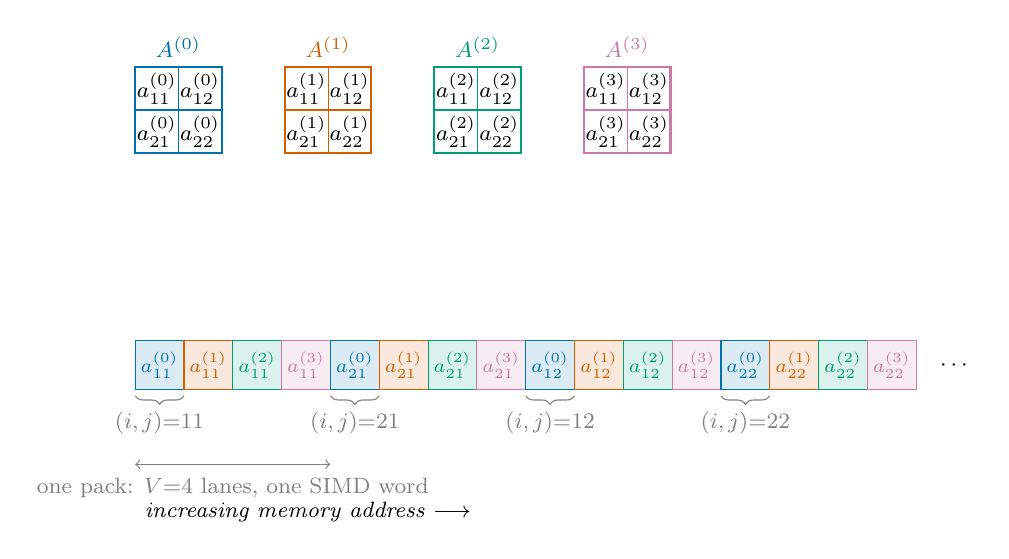
\begin{tikzpicture}[scale=1.0, font=\footnotesize]
  % --- the V=4 source matrices (2x2), colour-coded -----------------------
  \def\mats{{"matA","matB","matC","matD"}}
  \foreach \v/\col/\lab in {0/matA/0, 1/matB/1, 2/matC/2, 3/matD/3} {
     \begin{scope}[shift={(\v*1.9,3.0)}]
        \draw[\col,thick] (0,0) rectangle (1.1,1.1);
        \draw[\col] (0,0.55)--(1.1,0.55); \draw[\col] (0.55,0)--(0.55,1.1);
        \node at (0.275,0.82){$a^{(\lab)}_{11}$}; \node at (0.825,0.82){$a^{(\lab)}_{12}$};
        \node at (0.275,0.27){$a^{(\lab)}_{21}$}; \node at (0.825,0.27){$a^{(\lab)}_{22}$};
        \node[\col] at (0.55,1.35){$A^{(\lab)}$};
     \end{scope}
  }
  % --- the interleaved memory strip --------------------------------------
  % column-major element order within a matrix: (1,1),(2,1),(1,2),(2,2)
  \def\elems{{"11","21","12","22"}}
  \foreach \e/\elab in {0/{11}, 1/{21}, 2/{12}, 3/{22}} {
     \foreach \v/\col in {0/matA, 1/matB, 2/matC, 3/matD} {
        \pgfmathtruncatemacro{\idx}{\e*4+\v}
        \draw[\col,fill=\col!14] (\idx*0.62,0) rectangle (\idx*0.62+0.62,0.62);
        \node[\col] at (\idx*0.62+0.31,0.31){\scriptsize $a^{(\v)}_{\elab}$};
     }
     % element-group bracket + label
     \draw[decorate,decoration={brace,amplitude=3pt},gray]
        (\e*4*0.62+0.62,-0.08) -- (\e*4*0.62,-0.08);
     \node[gray] at (\e*4*0.62+0.31,-0.42){$(i,j){=}\elab$};
  }
  \node[anchor=west] at (10.1,0.31){$\cdots$};
  \draw[<->,gray] (0,-0.95) -- (2.48,-0.95);
  \node[gray,anchor=north] at (1.24,-1.0){one pack: $V{=}4$ lanes, one SIMD word};
  \node[anchor=west] at (0,-1.55){\itshape increasing memory address $\longrightarrow$};
\end{tikzpicture}
\caption{The compact / interleaved-batch layout for a pack of $V{=}4$ matrices of
order $2$ (column-major). The $V$ copies of each element $(i,j)$ occupy $V$
contiguous words, so a single $V$-wide SIMD load gathers the same element of all
$V$ matrices, and a scalar kernel becomes a batched one by widening its scalars
to vectors.}
\label{fig:interleave}
\end{figure}

This differs from the other common batched convention, the \emph{pointer array}
of BBLAS~\cite{bblas2021}, in which each matrix keeps its ordinary dense layout
and the batch is an array of pointers. Pointer arrays impose no repacking and
suit routines (like batched GEMM) whose per-matrix work is already large enough
to vectorize internally; the interleaved layout instead extracts parallelism
\emph{across} matrices, which is precisely what wins when each matrix is far too
small to fill a vector register on its own. The cost is a pack/unpack step at
the batch boundary (MKL's \code{mkl\_?gepack\_compact}/\code{geunpack\_compact});
in the target applications the same factored batch is reused enough --- across
right-hand sides, time steps, or Newton iterations --- to amortize it.

% =============================================================================
\section{Two vendor APIs, side by side}
\label{sec:vendors}

\begin{table}[t]
\centering
\caption{The compact/interleaved APIs and \cqr{}. \cqr{} follows MKL's calling
convention so it can substitute for, or interoperate with, MKL's own compact
routines, while remaining ISA-portable.}
\label{tab:apis}
\small
\begin{tabularx}{\linewidth}{@{}l l l X@{}}
\toprule
 & \textbf{MKL Compact} & \textbf{ArmPL interleave-batch} & \textbf{\cqr{} (this work)} \\
\midrule
Layout handle   & \code{MKL\_COMPACT\_PACK} (opaque $V$) & explicit inner/outer/batch strides & \code{MKL\_COMPACT\_PACK} \emph{or} explicit width $V$ \\
QR factor       & \code{mkl\_?geqrf\_compact}            & \code{armpl\_?geqrf\_interleave\_batch} & \code{cqr\_mkl\_?geqrf\_compact} \\
Apply $Q$       & \textbf{--- (absent)}                  & \code{armpl\_?ormqr\_interleave\_batch} & \code{cqr\_mkl\_?ormqr\_compact} \\
Triangular solve& \code{mkl\_?trsm\_compact}             & \code{armpl\_?trsm\_interleave\_batch}  & (use the vendor's) \\
Precisions      & s,d,c,z                                & s,d,c,z                                 & s,d (real only) \\
Target ISA      & x86 (SSE/AVX/AVX-512)                  & AArch64 (NEON/SVE)                      & any (single vector-typed source) \\
Source          & closed                                 & closed                                  & open (BSD-style)\\
\bottomrule
\end{tabularx}
\draftnote{verify exact ArmPL routine names/signatures against the current ArmPL reference.}
\end{table}

\paragraph{Intel MKL Compact.}
MKL hides the interleave width behind an opaque \code{MKL\_COMPACT\_PACK} token
obtained from \code{mkl\_get\_format\_compact()}, and pairs pack/unpack helpers
with a handful of compact BLAS/LAPACK kernels~\cite{mkl-compact}. For QR it
provides the factorization and the triangular solve but, as
Table~\ref{tab:apis} records, \emph{no} apply-$Q$: a caller can obtain the
reflectors $(H,\tau)$ and can do a triangular solve, but cannot form
$Q^{\mathsf T}B$ through a supported call. MKL's compact routines also skip
argument checking ``for performance reasons'' and leave \code{info}
reserved~\cite{mkl-compact}, and they document explicit numerical limitations ---
notably no safe handling of values near underflow/overflow, and no
pivoting~\cite{mkl-compact-limits}.

\paragraph{Arm Performance Libraries interleave-batch.}
ArmPL exposes the same idea with a more explicit hand: the caller passes inner,
outer, and batch strides describing the interleave directly~\cite{armpl-interleave},
which is more flexible but couples client code to the layout. Crucially for the
QR pipeline, ArmPL \emph{does} provide an interleaved apply-$Q$.

\paragraph{\cqr{}.}
\cqr{} adopts MKL's convention --- the opaque \code{MKL\_COMPACT\_PACK} token and
the identical argument list --- so a call site can swap \code{mkl\_?geqrf\_compact}
for \code{cqr\_mkl\_?geqrf\_compact} without change, and \cqr{}'s output feeds
MKL's \code{trsm\_compact} unmodified. It also exposes a second, MKL-free C API
taking the width $V$ explicitly, for use where MKL is not present. And it fills
the apply-$Q$ hole with \code{cqr\_mkl\_?ormqr\_compact}. The one thing it does
not inherit from either vendor is the ISA lock (below).

% =============================================================================
\section{\cqr{}: an open, portable reference implementation}
\label{sec:cqr}

\paragraph{One source, every width.}
\cqr{}'s central decision is to write each kernel once, over a scalar type
\code{T} and an interleave width \code{V}, using GNU vector types
(\code{\_\_attribute\_\_((vector\_size)))}. The compiler lowers that single
source to SSE, AVX, or AVX-512 on x86 --- and to NEON or SVE on AArch64 --- with
no per-ISA intrinsics. A thin dispatcher maps the runtime
\code{MKL\_COMPACT\_PACK} (or an explicit width) to the compile-time \code{V}
that selects the specialization. This is what lets one code base stand in for two
vendors' closed kernels.

\paragraph{Vectorized unblocked Householder QR.}
The factorization is the unblocked LAPACK algorithm \code{geqr2}
(\code{larfg} to build each reflector, \code{larf} to apply it to the trailing
columns~\cite{lapack-ug,golub2013}), run $V$ matrices at a time. Because the
compact layout makes element $(i,j)$ of all $V$ matrices contiguous
(Figure~\ref{fig:interleave}), the scalar algorithm lifts to SIMD by widening
\code{double} to a $V$-wide vector: every $+,-,\times,\div$ becomes a lane-wise
operation over $V$ independent matrices. The \emph{blocked} algorithm
(\code{geqrf}, with \code{larft}/\code{larfb}) is deliberately \emph{not} used:
at these orders the reflector panels are short, and the interleaved batch already
saturates the vector units without the extra bookkeeping. Column-major is the
tuned path --- a matrix column is contiguous in the compact buffer, so the norm
reduction, the reflector scaling, and the trailing-column update all walk
contiguous pointers, register-blocked a few trailing columns at a time.

\paragraph{The one hard part: a branch-free \code{larfg}.}
Scalar \code{larfg} contains a data-dependent branch (if the below-diagonal norm
is zero, $\tau=0$) and scalar special functions. Across a pack that branch would
diverge per lane, so it is rewritten branch-free with a mask and a select, keyed
on the LAPACK-correct quantity (the \emph{below-diagonal} norm, so an
already-triangular column yields $\tau=0$ with the diagonal untouched, exactly as
\code{larfg} does):

\begin{lstlisting}
tail  = sum_{i>k} A(i,k)^2            // vector reduction below the diagonal
x0    = A(k,k)
norm  = sqrt(x0*x0 + tail)            // == hypot(x0, ||tail||)
beta  = (x0 >= 0) ? -norm : norm      // -copysign(norm, x0), branch-free
has   = tail > 0                      // lane mask: is there anything to zero?
tau   = has ? (beta - x0)/beta : 0
inv   = has ? 1/(x0 - beta)     : 0   // masked select kills 0/0 and 1/0
A(k,k)     = has ? beta : x0          // R diagonal (unchanged if no tail)
A(i>k,k)  *= inv                      // reflector body (0*inv = 0 when !has)
\end{lstlisting}

\noindent
Only \code{sqrt} needs a helper --- a short lane loop that both GCC and Clang
lower to a single \code{vsqrt} --- while the comparison yields a native mask and
the select is a bit-blend. Every step is $O(1)$ per column; the $O(n^2)$
reductions and $O(n^3)$ trailing update are pure vector arithmetic. The same
\code{has} mask that makes an already-triangular column a no-op also neutralizes
the identity matrices that padding puts in the unused lanes of a partial final
pack, so the kernel runs unmasked at full width without ever producing a
\code{NaN}.

\paragraph{The remainder ``staircase''.}
Because work is organized around the width $V$ and a small register-blocking
factor, orders $n$ that are not multiples of those quantities leave a partial
tile whose cleanup is proportionally more expensive at small $n$. The sustained
rate therefore climbs in a gentle staircase rather than a smooth curve
(Figure~\ref{fig:gflops}); the effect is most visible at the smallest orders and
is exactly why the benchmark includes non-power sizes drawn from real stencils.

\paragraph{Completing the pipeline and its scope.}
With \code{cqr\_mkl\_?ormqr\_compact} supplying the apply-$Q$ step, the three
routines factor and solve a batched least-squares/linear system end to end ---
\code{geqrf\_compact} $\to$ \code{ormqr\_compact}$(\,'L','T'\,)$ $\to$
\code{trsm\_compact} --- the last borrowed from the vendor. Table~\ref{tab:coverage}
summarizes coverage. By design \cqr{} is real-precision only, performs no
argument checking on the MKL-style surface (like MKL), does not pivot (pivoting
needs comparisons that do not vectorize across a pack), and does not implement
\code{larfg}'s underflow/overflow rescaling --- the same limitation MKL documents
for its compact QR~\cite{mkl-compact-limits}.

\begin{table}[t]
\centering
\caption{\cqr{} feature coverage. The tuned contiguous kernel serves the
column-major, left-apply solver path; the other layout/side combinations run
through a correctness-first stride-generalized kernel over the same math.}
\label{tab:coverage}
\small
\begin{tabularx}{\linewidth}{@{}l X@{}}
\toprule
Precisions        & single (\code{s}), double (\code{d}); real only \\
Layouts           & column-major (tuned), row-major (stride-generalized) \\
\code{geqrf}      & vectorized unblocked \code{geqr2}, branch-free \code{larfg} \\
\code{ormqr}      & side $\in\{L,R\}$, trans $\in\{N,T\}$ ($C$ folds to $T$) \\
\code{potrf}      & designed (batched Cholesky); not yet implemented \\
Checking          & none on the MKL-style API; LAPACK-style \code{info}$=-j$ on the portable C API \\
Not supported     & complex (\code{c},\code{z}); column pivoting; underflow/overflow rescaling \\
\bottomrule
\end{tabularx}
\end{table}

% =============================================================================
\section{Experimental methodology}
\label{sec:method}

\draftnote{This section states the intended protocol; fill the two machine
specifications and confirm the details match the runs that produce the data.}

\paragraph{Machines.}
\textbf{x86:} \draftnote{CPU model, base/all-core clock, cores used, L2/L3, MKL
version, GCC/Clang version and flags (e.g.\ \code{-O3 -march=native}).}
\textbf{Arm:} \draftnote{AArch64 CPU, SVE vector length, cores, ArmPL version,
compiler and flags.}

\paragraph{Workload.}
Each data point factors a pool of \draftnote{$n_m$ (e.g.\ 512)} random,
well-conditioned square matrices of a fixed order $n$, in double precision. The
size list spans the target range and deliberately mixes powers of two with the
non-power stencil sizes $30,45,60,105,168$ (Section~\ref{sec:apps}) so the
remainder staircase is visible: $\{8,16,24,30,32,45,48,60,64,96,105,128,168,170,256,384,500\}$.

\paragraph{What is timed.}
The pool is packed into compact form \emph{once}, up front; only the
factorization is timed, and the destroyed input is restored (untimed) before each
pass. Reported times are the best of \draftnote{$r$} passes. The two compact
paths (\cqr{}, vendor) are driven from an outer parallel loop over packs --- the
intended usage --- with the vendor library's own threading pinned to one thread;
the per-matrix LAPACK baseline parallelizes over matrices the same way. This
isolates the factorization \emph{kernel}, not pack/unpack or data movement.

\paragraph{Correctness gate.}
Every timed configuration is checked (untimed) against per-matrix
\code{LAPACKE\_?geqrf}: the unpacked $(H,\tau)$ must match elementwise to a tight
tolerance, so each benchmark row doubles as an integration test. Reported
\code{relerr} is this quantity.

\paragraph{Reproducibility.}
The \cqr{} x86 numbers come from the repository's \code{bench\_geqrf\_compact}
driver; the ArmPL numbers require the AArch64 harness described in
Section~\ref{sec:future}. Scripts, data, and this document build with a single
\code{make} (see the report \code{README}).

% =============================================================================
\section{Results}
\label{sec:results}

\begin{center}\fbox{\parbox{0.94\linewidth}{\centering
\draftnote{All figures below use \textbf{synthetic placeholder data}
(\code{report/data/*.dat}). They exist to validate the plotting pipeline and the
narrative shape; replace them with measured runs before drawing any conclusion.
See \code{report/data/README.md}.}}}\end{center}

\paragraph{Throughput on x86 (vs MKL Compact).}
Figure~\ref{fig:tput-x86} plots throughput (matrices/s) against order for \cqr{},
\code{mkl\_?geqrf\_compact}, and the per-matrix LAPACK loop. The expected pattern,
and the one the project reports on its AVX-512 test machine, is that both compact
paths dominate the per-matrix loop across the small-size range --- where
cross-matrix SIMD is the only way to fill the vector units --- and that \cqr{}
leads MKL at the smallest orders, the two converging as $n$ grows and per-matrix
internal vectorization begins to pay for the vendor kernel.
Figure~\ref{fig:speedup-x86} shows the same story as speedups over the per-matrix
baseline, with the crossover made explicit. \draftnote{state the geometric-mean
speedup and the crossover order once measured.}

\begin{figure}[t]
\centering
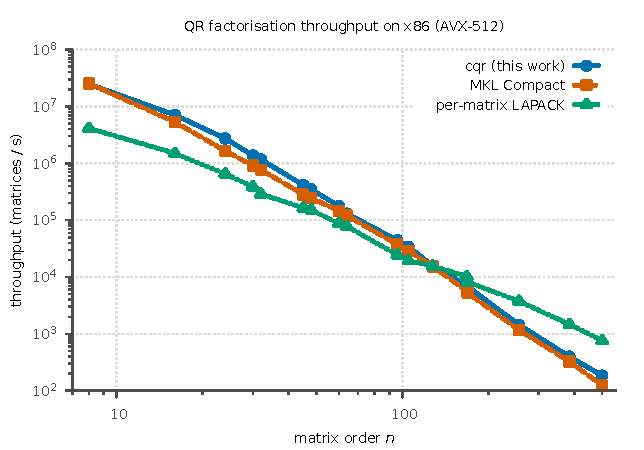
\includegraphics[width=0.72\linewidth]{figures/throughput_x86.pdf}
\caption{Batched QR factorization throughput on x86 (AVX-512): \cqr{} vs MKL
Compact vs a per-matrix LAPACK loop, over the target size range.
\emph{Placeholder data.}}
\label{fig:tput-x86}
\end{figure}

\begin{figure}[t]
\centering
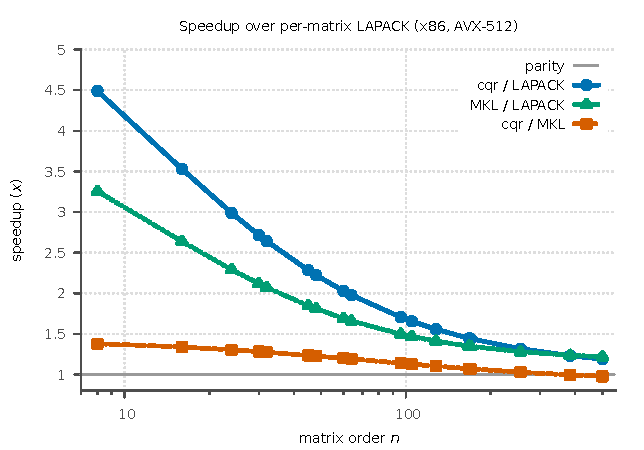
\includegraphics[width=0.72\linewidth]{figures/speedup_x86.pdf}
\caption{Speedup over the per-matrix LAPACK baseline on x86. The batched
advantage is largest at the smallest orders and narrows toward the parity line as
$n$ grows. \emph{Placeholder data.}}
\label{fig:speedup-x86}
\end{figure}

\paragraph{Throughput on Arm (vs ArmPL interleave-batch).}
Figure~\ref{fig:tput-arm} repeats the comparison on AArch64 against ArmPL's
interleave-batch \code{geqrf}. The question here is the \emph{portability tax}:
how close does a single vector-typed source come to a vendor kernel hand-tuned
for SVE? \draftnote{report the observed gap; note where \cqr{} leads (smallest
orders) and where ArmPL's tuning pulls ahead.}

\begin{figure}[t]
\centering
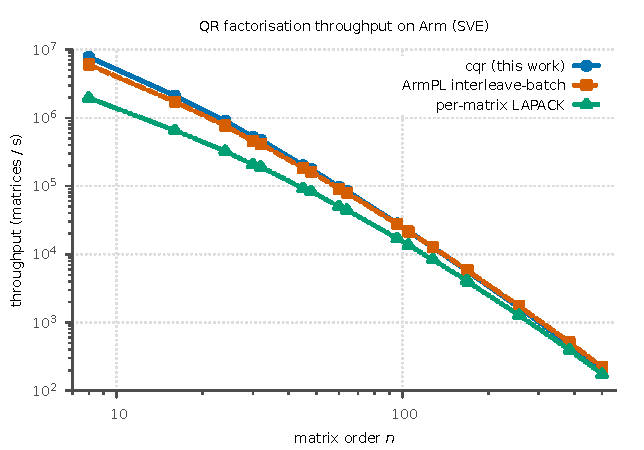
\includegraphics[width=0.72\linewidth]{figures/throughput_arm.pdf}
\caption{Batched QR factorization throughput on Arm (SVE): \cqr{} vs ArmPL
interleave-batch vs a per-matrix LAPACK loop. \emph{Placeholder data.}}
\label{fig:tput-arm}
\end{figure}

\paragraph{Sustained rate and the staircase.}
Figure~\ref{fig:gflops} plots \cqr{}'s sustained GFLOP/s on both machines. Two
features matter: the rate climbs and saturates as $n$ grows (better vector-unit
utilization), and it does so in a gentle staircase, dipping at orders that are
not multiples of the interleave width --- the remainder effect of
Section~\ref{sec:cqr}, and the reason the size list includes the odd stencil
sizes.

\begin{figure}[t]
\centering
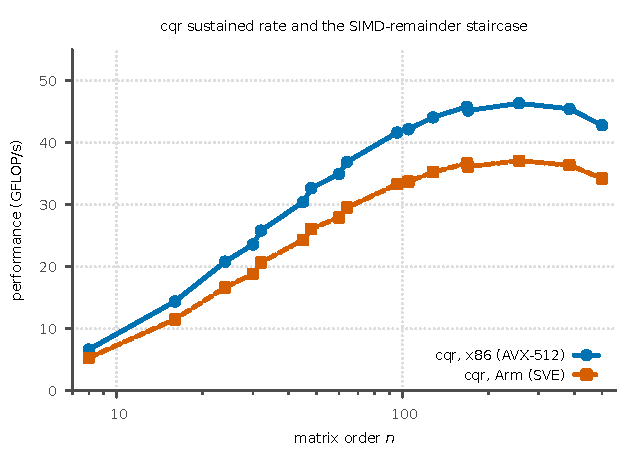
\includegraphics[width=0.72\linewidth]{figures/gflops.pdf}
\caption{\cqr{} sustained rate (GFLOP/s) vs order on x86 and Arm. The wiggle at
non-multiple-of-$V$ orders is the SIMD-remainder staircase. \emph{Placeholder data.}}
\label{fig:gflops}
\end{figure}

% =============================================================================
\section{Discussion and limitations}
\label{sec:discussion}

The results (once measured) speak to a specific claim: that the interleaved
format's advantage comes from the \emph{layout}, not from any vendor's closed
microkernel, and can therefore be had portably. If \cqr{} tracks MKL on x86 and
ArmPL on Arm from one source, the format --- not the implementation --- is doing
the work, and there is no reason for it to remain closed or ISA-locked.

The scope limits are deliberate and mirror the vendors'. \cqr{} is real-only;
complex Hermitian QR is future work. It does not pivot, so it is unsuited to
rank-revealing factorizations --- but the target least-squares and interpolation
problems are set up to be well conditioned. It omits \code{larfg}'s
underflow/overflow rescaling, matching MKL's documented compact
limitation~\cite{mkl-compact-limits}; inputs scaled to the exponent extremes are
out of scope. And the row-major and right-apply paths are correctness-first, not
separately SIMD-tuned: the tuned path is the column-major, left-apply solver
route the applications use.

% =============================================================================
\section{Related work}
\label{sec:related}

The batched-BLAS effort defined the problem and a pointer-array interface
standard~\cite{bblas2021,bblas-standard}. The interleaved/compact layout is the
vendors' alternative for the small-matrix regime: Intel's Compact
functions~\cite{mkl-compact} and Arm's interleave-batch
functions~\cite{armpl-interleave}. Portable batched kernels also appear in
Kokkos Kernels~\cite{kokkos-kernels}, and the \code{batmat} project~\cite{batmat}
provides interleaved batched linear algebra aimed at convex optimization. \cqr{}'s
contribution relative to these is narrow and specific: an \emph{open} drop-in for
the MKL compact QR that is portable across ISAs from one source and that supplies
the apply-$Q$ step MKL omits. \draftnote{if targeting a venue, add the closest
compact-QR performance papers and any batched-QR-on-GPU comparison for context.}

% =============================================================================
\section{Conclusion and future work}
\label{sec:future}

The compact/interleaved format is the right data structure for batches of many
small identically-shaped matrices, and it is architecture-neutral even though
today's implementations are closed and ISA-locked. \cqr{} shows the format can be
served by a single portable, vector-typed source that stands in for
\code{mkl\_?geqrf\_compact}, completes the pipeline MKL leaves open, and is meant
to match both vendors' kernels in the size range the motivating applications ---
meshless approximation and multi-physics data mapping --- actually use.

Future work: (i) the AArch64/ArmPL benchmark harness needed to turn
Figure~\ref{fig:tput-arm} into measured results --- building \cqr{} so the vector
types lower to NEON/SVE, and a driver that bridges ArmPL's stride-based
interleave to the compact packs; (ii) the batched Cholesky
\code{cqr\_mkl\_?potrf\_compact}, already specified, for the normal-equations form
of the MLS/RBF problems; (iii) complex precisions; and (iv) an end-to-end
application benchmark (an RBF-FD weight assembly) rather than the kernel
microbenchmark alone.

\section*{Availability}
\draftnote{repository URL, licence, and archived release DOI (e.g.\ Zenodo) for a
citable artifact.}

\section*{Acknowledgements}
\draftnote{funding, compute resources, and any tool/assistance acknowledgements
consistent with the project's conventions.}

\bibliographystyle{plainnat}
\bibliography{refs}

\end{document}
